\documentclass[a4paper,oneside,article,11pt]{memoir}
\usepackage[english]{babel}
\usepackage[utf8]{inputenc}
\usepackage{amsmath,amssymb,amsthm}

% This font looks so good.
\usepackage[sc]{mathpazo}

% Typesetting pseudo-code
\usepackage{algorithm}
\usepackage{algorithmic}
\usepackage{multirow}
% Code comments like [CLRS]
\renewcommand{\algorithmiccomment}[1]{\makebox[5cm][l]{$\triangleright$ \textit{#1}}}
\usepackage{framed,graphicx,xcolor}
\usepackage[font={small,it}]{caption}
\usepackage{listings}
\usepackage{units}

% Relative references
\usepackage{varioref}

\usepackage{hyperref}

\bibliographystyle{plain}

\title{Advanced Data Structures \\ Project 1 - Fibonacci heaps}
\author{Peter Gabrielsen 20114179 \\
Christoffer Hansen 20114637}
\newcounter{qcounter}
\begin{document}

\begin{titlingpage}
\clearpage

\maketitle
\thispagestyle{empty}

\begin{abstract}
ABSTRACT HERE
\\
\\
\\
The code can be found at: \\\url{CODE HERE}.
\end{abstract}
\end{titlingpage}

\pagebreak

\tableofcontents

\pagebreak

\chapter{Introduction}
INTRO

\chapter{Implementation}
We will in this section describe and discuss the design choices of our implementations of the binary heap and the Fibonacci heap.
\subsection{Binary heap}

\subsection{Fibonacci heap}

\chapter{Experimental setup}
\label{chtp:experiment_setup}
%TODO write something about the machine which ran the experiments and something about how we measure the different things. Maybe copy all this from the AE report?

The experiments were performed on a machine with a Intel i5-3210M @ 2.5GHz (Ivy Bridge) with 128K bytes of L1 cache, 512K bytes of L2 and 3072K bytes of L3 cache. The machine had 4.2GB ram and ran Ubuntu 14.04 with kernel version 3.16.0-50.

The running time was measured using the built in \texttt{high\_resolution\_clock} in the \texttt{chrono} library. This measures the wall clock. It is the clock in \texttt{c++} with the highest precision, i.e. the shortest tick period.

The code is compiled with \texttt{g++ 4.8.4} with the \texttt{c++11} standard enabled and no optimization level.

The elements in our data structures were 32 bit integers. Random elements were generated uniformly in the 32 bit integer range using the Mersenne Twister 19937 from the \texttt{random} library.

CPU measurements were collected using \texttt{PAPI 5.3.0.0}

We used \texttt{perf} to measure page faults.


\chapter{Worst case time bounds of the heaps}
In this section we will argue about how the algorithms perform in the worst case as opposed to the amortized time bounds. We will for each operations on the heaps argue how the worst cases are obtained.

\subsection{FindMin}
Finding the minimum element is in both the Fibonacci heap and the binary heap a constant time operation. We keep a pointer to the minimum element in the Fibonacci heap and in the binary heap we just return the first element in the array which holds the heap.

\subsection{Insert}
Inserting into the binary heap is simple. We insert the element at the last position in the binary tree, i.e. the heap, and bubble the element up to its correct position. In the worst case we need to bubble the element to the top, which means bubbling through $\mathcal{O}(\log n)$ layers which gives a logarithmic complexity in the worst case for this operation.

Inserting in the Fibonacci heap is even simpler. We simply just add the element to the root list which just involves manipulating a doubly linked list, i.e. some pointer calculations. 
%This constant time operation is what allows us to give the amortized analysis of decrease key?

\subsection{DeleteMin}
Delete the minimum element is $\mathcal{O}(\log{n})$ for the binary heap and $\mathcal{O}(\log{n})$ amortized for the Fibonacci heap. This upper bound is trivially obtained in the binary heap by having the heap ordered as a sorted array. This way, whenever we delete the minimum we would move the largest element to the top and bubble it $\log n$ levels down again to the bottom.

It can however be extremely expensive to delete the minimum in the Fibonacci heap. When we delete the minimum from a Fibonacci heap we need to consolidate the heap. This operations is linear in the size of the root list. The root list can grow linearly in the worst case if we do $n$ inserts in a row, then the root list will contain at least $n$ nodes, which needs to be consolidated in time $\mathcal{O}(\vert root\_list \vert)$.

\subsection{DecreaseKey}
Decreasing a key in the binary heap is done by giving the element a new priority and then bubble it up to its new position. The worst case is that the element decreased is the last element and its new priority is the lowest in the tree, which means that it needs to bubble to the top of the heap. This costs $\mathcal{O}(\log n)$.

The worst case for the Fibonacci heap would be if we have a tree of height $\mathcal{O}(\log n)$ where every internal node on the path to the lowest leaf, which is decreased, is marked. This will cause a chain of cuts and cascading cuts all the way up to the root, which will take $\mathcal{O}(\log n)$ time.

\chapter{Heap experiments}
In this section we will design and perform experiments where we try to measure the running time and number of comparisons of the operations for both our priority queue implementations. We will give a summary of the design of each experiment, results, and discussion of the found results for each operation.

\subsection{FindMin}
Since finding the minimum element of both queues are constant time operations and basically just dereferencing a pointer we did not think it made sense to compare the running times in terms of wall clock. What we did instead is we measured the number of cycles for performing a single FindMin operation and the number of conditional branching operations needed. We would highly expect that the results do not depend on the size of the heap, why we made an experiment where the size of the heap was powers of two in the range from $\left[2^0, 2^{22}\right]$. The results can be found in figure~\ref{fig:findmin_cycles} and figure~\ref{fig:findmin_cr}.
Our hypothesis was fortunately true and we do not think that there is much to discuss about the results.

\subsection{Insert}
Inserting in the Fibonacci heap is a constant time operation while inserting into the binary heap is logarithmic. We would like to see that the binary heap performs worse. We will test both priority queues in both the average case and the worst case. In the average case we select a random priority in the integer range and insert it into the heap.
%TODO how high can we expect the elemen to bubble on average?
In the worst case we insert elements into the heap in reverse order. This will cause the elements to bubble all the way to the top on every insert.

We expect to see that the Fibonacci heap is constant time in any case and that the binary heap is logarithmic in both cases. The number of comparisons performed in the Fibonacci heap should therefore also be constant on each insert while the number of comparisons should increase logarithmically in the size of the input.

The results can be found in figure~\ref{fig:insert_t},~\ref{fig:insert_c}.

%TODO Add discussion of the results here!


\subsection{DeleteMin}
Deleting the minimum element takes logarithmic time both priority queues. It can however take linear time in the worst case for the Fibonacci queue if a delete minimum operation is performed right after $n$ insert operations. We measure deleting the minimum in the average case where we randomly insert $n$ elements and then first pop one element from both queues such that the Fibonacci queue has consolidated. We then measure the on deleting one element for different heap sizes. We expect to see both have a logarithmic running time and comparisons.
Testing in the worst case we will do the same but not consolidate the Fibonacci heap first and the binary heap should be inserted in sorted order.

The results can be found in figure~\ref{fig:delmin_c} and \ref{fig:delmin_t}.

%TODO add discussion of results.


%TODO compiling using O2 makes bh better than fh but not in worst case MSP

\chapter{Dijkstra's algorithm}
In this section we introduce families of graphs that we believe makes Dijkstra's algorithm perform many respectively few \texttt{DecreaseKey} operations. It is obvious that the number of \texttt{DecreaseKey} operations is an exact measure of the number of edges we have to \textit{relax}.

\section{Few \texttt{DecreaseKey} operations}
\label{sec:few_decreasekey}
Since Dijkstra's algorithm finds shortest paths from the source $s$ to all vertices in the graph, we have to relax at least one ingoing edge for all other vertices. We therefore conclude that the lower bound for relaxing edges must be $\vert V \vert -1$. If not, the graph would contain unvisited vertices. Having a chain of vertices with \textit{weight} 0 on all edges causes Dijkstra to \textit{relax} each edge exactly once, giving us a graph with the desired property. It is clear that no additional (positive weighted) edges will be relaxed. For a graphical representation of the described class of graphs, please to figure~\ref{figure:graph_chain}. For future reference we denote this family of graphs \texttt{ChainGraphs}.

\begin{figure}[H]
\centering
\centerline {
  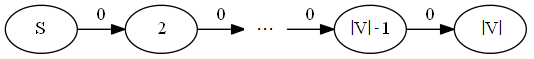
\includegraphics[scale=1]{../figures/graph_chain.png}
}
\caption{Chain of $\vert V \vert$ nodes with edge weight 0.}
\label{figure:graph_chain}
\end{figure}

\section{Many \texttt{DecreaseKey} operations}
\label{sec:many_decreasekey}
We consider an analysis of Dijkstra's algorithm using the fact that our implementation makes use of a priority queue $Q$. Since each vertex is removed from $Q$ exactly once, and the adjacency list of each vertex is scanned exactly once, it is clear that we can at most relax all edges exactly once.
In other words we need to consider graphs that makes Dijkstra's algorithm perform $\vert E \vert$ \texttt{DecreaseKey} operations in order to reach the upper bound.

We present two candidates of classes of graphs with the above mentioned property. The first proposal makes use of negative weights. Dijkstra's algorithm would still be able to run since we are not introducing negative cycles, but as we allow for previously marked nodes to be reinserted into the priority queue, we cannot rely on the asymptotic time bound. The second proposal uses only positive edge weights, and can therefore be compared against the asymptotic analysis.

\subsection{Candidate 1}
In the first candidate we split $n$ vertices into two sets $S_1, S_2$ of sizes $\lceil \nicefrac{(n-1)}{2} \rceil$ and $\lfloor \nicefrac{(n-1)}{2} \rfloor$ respectively. We now construct a chain of vertices from $S_1$. For chained vertex $v_i$ we have outgoing edge weight equal to $i$ for all $i \in [1, .. ,\lvert S_1 \lvert - 1]$. The last vertex on the chain has no outgoing edges for now. We now connect each vertex $v_i$ on the chain to all vertices ${v'}_i$ in $S_2$ with edge weight equal to $-2 \cdot i$. Finally we connect the source $s$ to $v_1$ in the chain with edge weight $n$ and to all ${v'}_i \in S_2$ with edge weight $n-1$. Please refer to figure~\ref{figure:graph_neg_weights} for an example with $n=6$. It is clear the example will make Dijkstra's algorithm relax all edges, and that this fact generalizes to graphs of arbitrary sizes.

\begin{figure}[H]
\centering
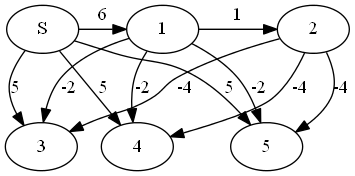
\includegraphics[scale=0.8]{../figures/graph_neg_weights.png}
\caption{Dijkstra's algorithm will have to relax all edges but we make us of negative edges}
\label{figure:graph_neg_weights}
\end{figure}

\subsection{Candidate 2}
In the second candidate we split $n$ vertices into three set $S_2, S_2$ and $S_3$ of sizes $\lceil \nicefrac{(n-1)}{3} \rceil$, $\lfloor \nicefrac{(n-1)}{3} \rfloor$ and $(n-1) - \lvert S_1 \rvert - \lvert S_2 \rvert$ respectively. We now construct a chain of vertices from $S_1$ with edge weight $0$. Connect each vertex $v_i$ on the chain to all vertices ${v''}_i \in S_3$ with edge weight equal to $n-2i$. Now connect each vertex ${v'}_i \in S_2$ to all vertices ${v''}_i \in S_3$ with edge weight $n^2 + 2n - 2i$ (we could have used $n^3$ for smaller $n$, but in order to avoid overflow we use this edge weight). Finally connect the source $s$ to the first vertex on the chain in $S_1$ with edge weight $n^2$ and to all vertices ${v'}_i \in S_2$ with edge weight $n+i$. Please refer to figure~\ref{figure:graph_pos_weights} for an example with $n=9$.  It is clear the example will make Dijkstra's algorithm relax all edges, and that this fact generalizes to graphs of arbitrary sizes. For future reference we denote this family of graphs \texttt{HeavyGraphs}

\begin{figure}[H]
\centering
\centerline {
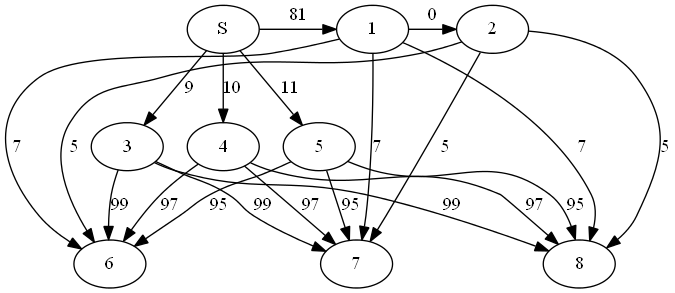
\includegraphics[scale=0.65]{../figures/graph_positive_weights.png}
}
\caption{Dijkstra's algorithm will have to relax all edges and we use only positive edges}
\label{figure:graph_pos_weights}
\end{figure}

\chapter{Experiments on Dijkstra's}
In this section we document the experiments done on Dijkstra's algorithm using both heap implementations. In particular we focus our studies on observing if the version using Fibonacci heaps achieves an improved performance because of the amortized $\mathcal{O}(1)$ time \texttt{DecreaseKey} operation. In the following we set $n = \lvert V \lvert$.

\section{Methodology}
We perform experiments using three families of graphs, namely \texttt{ChainGraphs} introduced in section~\ref{sec:few_decreasekey}, \texttt{HeavyGraphs} introduced in section~\ref{sec:few_decreasekey} and \texttt{RandomGraphs}. We will introduce the latter family in a short moment. Since we aim at comparing Dijkstra's algorithm on the different families, we started out by adding edges to the graphs such that they have equal number of edges on equal number of vertices. It is intuitively obvious that \texttt{HeavyGraphs} have more edges than \texttt{ChainGraphs}. A careful analysis tells us that graphs in \texttt{HeavyGraphs} with $\lvert V \rvert = n$ will have exactly $2(\nicefrac{n}{3})^2 + (\nicefrac{n}{3})-1$ edges. This gives reason for the following extensions of the constructions of each family.

\subsection{\texttt{ChainGraphs}}
We construct each graph as described in section~\ref{sec:few_decreasekey}. Furthermore we add $2(\nicefrac{n}{3})^2 + (\nicefrac{n}{3})- n - 2$ edges uniformly distributed over all vertices with edge weight $0$. This will make the graph have the desired total number of edges equal to graphs in \texttt{HeavyGraphs}. The extension will not make the graphs loose the property of making Dijkstra's algorithm perform few \texttt{DecreaseKey} operations.

\subsection{\texttt{HeavyGraphs}}
We construct each graph following the algorithm presented as \textit{Candidate 2} in section~\ref{sec:many_decreasekey}. Now further extensions is needed.

\subsection{\texttt{RandomGraphs}}
We construct each graph with $n$ vertices having $\dfrac{2(\nicefrac{n}{3})^2 + (\nicefrac{n}{3})-1}{n}$ outgoing edges. Each edge is connected uniformly random to another vertex. We avoid having edges connecting a vertex to itself and we avoid to have multiple outgoing edges to the same vertex. Edge weights are taken uniformly random in the interval $[0, .., 100]$. After construction we make sure that all components are connected. We do this by colouring all components and afterwards connecting different coloured components with a random edge. This scheme have a very limited overhead in number of extra edges.

\subsection{Experimental setup}
Please refer to chapter~\ref{chtp:experiment_setup} for a general overview of the experimental setup. Each experiment was performed ??? times and the average was used.

\section{Expectations}
fdsa

\section{Results}
dsaf

\section{Discussion}
fads

\bibliography{references}

\end{document}


